\documentclass{standalone}
\usepackage{tikz}
\usetikzlibrary{patterns, positioning}

\begin{document}
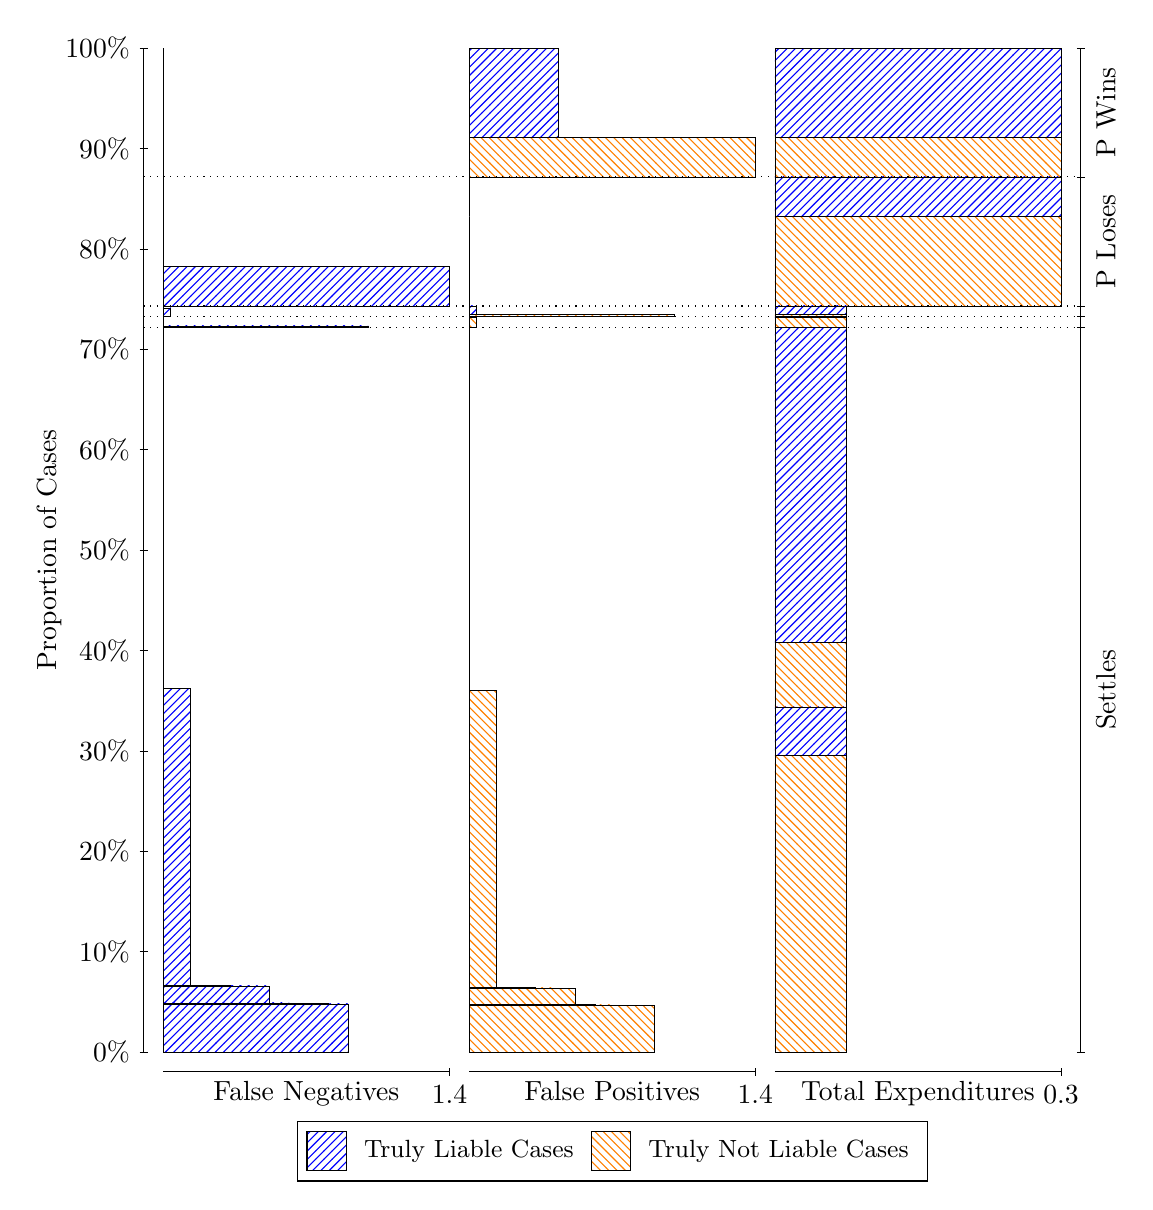
\begin{tikzpicture}
\draw[black, very thin] (1.5,1.75) -- (1.5,14.5);
\node[rotate=90, anchor=center] at (0.3, 8.125) {Proportion of Cases};
\draw[black, very thin] (1.45,1.75) -- (1.55,1.75);
\node[anchor=east] at (1.45, 1.75) {0\%};
\draw[black, very thin] (1.45,3.025) -- (1.55,3.025);
\node[anchor=east] at (1.45, 3.025) {10\%};
\draw[black, very thin] (1.45,4.3) -- (1.55,4.3);
\node[anchor=east] at (1.45, 4.3) {20\%};
\draw[black, very thin] (1.45,5.575) -- (1.55,5.575);
\node[anchor=east] at (1.45, 5.575) {30\%};
\draw[black, very thin] (1.45,6.85) -- (1.55,6.85);
\node[anchor=east] at (1.45, 6.85) {40\%};
\draw[black, very thin] (1.45,8.125) -- (1.55,8.125);
\node[anchor=east] at (1.45, 8.125) {50\%};
\draw[black, very thin] (1.45,9.4) -- (1.55,9.4);
\node[anchor=east] at (1.45, 9.4) {60\%};
\draw[black, very thin] (1.45,10.675) -- (1.55,10.675);
\node[anchor=east] at (1.45, 10.675) {70\%};
\draw[black, very thin] (1.45,11.95) -- (1.55,11.95);
\node[anchor=east] at (1.45, 11.95) {80\%};
\draw[black, very thin] (1.45,13.225) -- (1.55,13.225);
\node[anchor=east] at (1.45, 13.225) {90\%};
\draw[black, very thin] (1.45,14.5) -- (1.55,14.5);
\node[anchor=east] at (1.45, 14.5) {100\%};

\draw[black, very thin] (13.4,1.75) -- (13.4,14.5);
\draw[black, very thin] (13.35,1.75) -- (13.45,1.75);
\node[anchor=west] at (13.35, 1.75) {};
\draw[black, very thin] (13.35,10.952) -- (13.45,10.952);
\node[anchor=west] at (13.35, 10.952) {};
\draw[black, very thin] (13.35,11.094) -- (13.45,11.094);
\node[anchor=west] at (13.35, 11.094) {};
\draw[black, very thin] (13.35,11.224) -- (13.45,11.224);
\node[anchor=west] at (13.35, 11.224) {};
\draw[black, very thin] (13.35,12.864) -- (13.45,12.864);
\node[anchor=west] at (13.35, 12.864) {};
\draw[black, very thin] (13.35,14.5) -- (13.45,14.5);
\node[anchor=west] at (13.35, 14.5) {};

\draw[black, very thin, pattern color=blue, pattern=north east lines] (1.75,1.75) rectangle (4.0991,2.3614);
\draw[black, very thin, pattern color=blue, pattern=north east lines] (1.75,2.3614) rectangle (3.8486,2.3655);
\draw[black, very thin, pattern color=blue, pattern=north east lines] (1.75,2.3655) rectangle (3.598,2.3698);
\draw[black, very thin, pattern color=blue, pattern=north east lines] (1.75,2.3698) rectangle (3.3474,2.374);
\draw[black, very thin, pattern color=blue, pattern=north east lines] (1.75,2.374) rectangle (3.0968,2.5881);
\draw[black, very thin, pattern color=blue, pattern=north east lines] (1.75,2.5881) rectangle (2.8463,2.59);
\draw[black, very thin, pattern color=blue, pattern=north east lines] (1.75,2.59) rectangle (2.5957,2.592);
\draw[black, very thin, pattern color=blue, pattern=north east lines] (1.75,2.592) rectangle (2.3451,2.594);
\draw[black, very thin, pattern color=blue, pattern=north east lines] (1.75,2.594) rectangle (2.0945,6.3639);
\draw[black, very thin, pattern color=orange, pattern=north west lines] (1.75,6.3639) rectangle (1.75,10.952);
\draw[black, very thin, pattern color=blue, pattern=north east lines] (1.75,10.952) rectangle (4.3497,10.971);
\draw[black, very thin, pattern color=orange, pattern=north west lines] (1.75,10.971) rectangle (1.75,11.094);
\draw[black, very thin, pattern color=blue, pattern=north east lines] (1.75,11.094) rectangle (1.844,11.2);
\draw[black, very thin, pattern color=orange, pattern=north west lines] (1.75,11.2) rectangle (1.75,11.224);
\draw[black, very thin, pattern color=blue, pattern=north east lines] (1.75,11.224) rectangle (5.3833,11.729);
\draw[black, very thin, pattern color=orange, pattern=north west lines] (1.75,11.729) rectangle (1.75,12.864);
\draw[black, very thin, pattern color=orange, pattern=north west lines] (1.75,12.864) rectangle (1.75,13.37);
\draw[black, very thin, pattern color=blue, pattern=north east lines] (1.75,13.37) rectangle (1.75,14.5);
\draw[black, very thin, pattern color=orange, pattern=north west lines] (5.6333,1.75) rectangle (7.9825,2.3438);
\draw[black, very thin, pattern color=orange, pattern=north west lines] (5.6333,2.3438) rectangle (7.7319,2.3462);
\draw[black, very thin, pattern color=orange, pattern=north west lines] (5.6333,2.3462) rectangle (7.4813,2.3485);
\draw[black, very thin, pattern color=orange, pattern=north west lines] (5.6333,2.3485) rectangle (7.2307,2.3507);
\draw[black, very thin, pattern color=orange, pattern=north west lines] (5.6333,2.3507) rectangle (6.9802,2.5599);
\draw[black, very thin, pattern color=orange, pattern=north west lines] (5.6333,2.5599) rectangle (6.7296,2.5599);
\draw[black, very thin, pattern color=orange, pattern=north west lines] (5.6333,2.5599) rectangle (6.7296,2.565);
\draw[black, very thin, pattern color=orange, pattern=north west lines] (5.6333,2.565) rectangle (6.479,2.5701);
\draw[black, very thin, pattern color=orange, pattern=north west lines] (5.6333,2.5701) rectangle (6.2284,2.575);
\draw[black, very thin, pattern color=orange, pattern=north west lines] (5.6333,2.575) rectangle (5.9779,6.3383);
\draw[black, very thin, pattern color=blue, pattern=north east lines] (5.6333,6.3383) rectangle (5.6333,10.952);
\draw[black, very thin, pattern color=orange, pattern=north west lines] (5.6333,10.952) rectangle (5.7273,11.075);
\draw[black, very thin, pattern color=blue, pattern=north east lines] (5.6333,11.075) rectangle (5.6333,11.094);
\draw[black, very thin, pattern color=orange, pattern=north west lines] (5.6333,11.094) rectangle (8.233,11.118);
\draw[black, very thin, pattern color=blue, pattern=north east lines] (5.6333,11.118) rectangle (5.7273,11.224);
\draw[black, very thin, pattern color=orange, pattern=north west lines] (5.6333,11.224) rectangle (5.6333,12.359);
\draw[black, very thin, pattern color=blue, pattern=north east lines] (5.6333,12.359) rectangle (5.6333,12.864);
\draw[black, very thin, pattern color=orange, pattern=north west lines] (5.6333,12.864) rectangle (9.2667,13.37);
\draw[black, very thin, pattern color=blue, pattern=north east lines] (5.6333,13.37) rectangle (6.7609,14.5);
\draw[black, very thin, pattern color=orange, pattern=north west lines] (9.5167,1.75) rectangle (10.425,5.5182);
\draw[black, very thin, pattern color=blue, pattern=north east lines] (9.5167,5.5182) rectangle (10.425,6.1337);
\draw[black, very thin, pattern color=orange, pattern=north west lines] (9.5167,6.1337) rectangle (10.425,6.9538);
\draw[black, very thin, pattern color=blue, pattern=north east lines] (9.5167,6.9538) rectangle (10.425,10.952);
\draw[black, very thin, pattern color=orange, pattern=north west lines] (9.5167,10.952) rectangle (10.425,11.075);
\draw[black, very thin, pattern color=blue, pattern=north east lines] (9.5167,11.075) rectangle (10.425,11.094);
\draw[black, very thin, pattern color=orange, pattern=north west lines] (9.5167,11.094) rectangle (10.425,11.118);
\draw[black, very thin, pattern color=blue, pattern=north east lines] (9.5167,11.118) rectangle (10.425,11.224);
\draw[black, very thin, pattern color=orange, pattern=north west lines] (9.5167,11.224) rectangle (13.15,12.359);
\draw[black, very thin, pattern color=blue, pattern=north east lines] (9.5167,12.359) rectangle (13.15,12.864);
\draw[black, very thin, pattern color=orange, pattern=north west lines] (9.5167,12.864) rectangle (13.15,13.37);
\draw[black, very thin, pattern color=blue, pattern=north east lines] (9.5167,13.37) rectangle (13.15,14.5);
\draw[black, dotted] (1.5,10.952) -- (13.4,10.952);
\draw[black, dotted] (1.5,11.094) -- (13.4,11.094);
\draw[black, dotted] (1.5,11.224) -- (13.4,11.224);
\draw[black, dotted] (1.5,12.864) -- (13.4,12.864);
\draw[black, very thin] (1.75,1.5) -- (5.3833,1.5);
\node[anchor=north] at (3.5667, 1.5) {False Negatives};
\draw[black, very thin] (5.3833,1.45) -- (5.3833,1.55);
\node[anchor=north] at (5.3833, 1.45) {1.4};

\draw[black, very thin] (5.6333,1.5) -- (9.2667,1.5);
\node[anchor=north] at (7.45, 1.5) {False Positives};
\draw[black, very thin] (9.2667,1.45) -- (9.2667,1.55);
\node[anchor=north] at (9.2667, 1.45) {1.4};

\draw[black, very thin] (9.5167,1.5) -- (13.15,1.5);
\node[anchor=north] at (11.333, 1.5) {Total Expenditures};
\draw[black, very thin] (13.15,1.45) -- (13.15,1.55);
\node[anchor=north] at (13.15, 1.45) {0.3};

\node[black, centered, rotate=90] at (13.72, 6.3511) {Settles};


\node[black, centered, rotate=90] at (13.72, 12.044) {P Loses};
\node[black, centered, rotate=90] at (13.72, 13.682) {P Wins};

\draw (7.449999999999999,1.5) node[draw=none] (baseCoordinate) {};
\begin{scope}[align=center]
        \matrix[scale=0.5, draw=black, below=0.5cm of baseCoordinate, nodes={draw}, column sep=0.1cm]{
            \node[rectangle, draw, minimum width=0.5cm, minimum height=0.5cm, pattern=north east lines, pattern color=blue] {}; &
            \node[draw=none, font=\small] (B) {Truly Liable Cases}; &
            \node[rectangle, draw, minimum width=0.5cm, minimum height=0.5cm, pattern=north west lines, pattern color=orange] {}; &
            \node[draw=none, font=\small] (B) {Truly Not Liable Cases}; \\
            };
\end{scope}

\end{tikzpicture}
\end{document}